% ---------------------------------------------------------------------------
% ---------------------------------------------------------------------------
% Modelo LaTex para preparação do documento final de Monografia TCC
% O modelo está em conformidade com ABNT NBR
% Faculdade do Piaui
% ---------------------------------------------------------------------------
% ---------------------------------------------------------------------------

\documentclass[
	% -- opções da classe memoir --
	12pt,					% tamanho da fonte
	book,				% capítulos começam em pág ímpar (insere página vazia caso preciso)
	oneside,					% para impressão em verso e anverso. Oposto a oneside
	a4paper,					% tamanho do papel. 
	% -- opções da classe abntex2 --
	%chapter=TITLE,			% títulos de capítulos convertidos em letras maiúsculas
	%section=TITLE,			% títulos de seções convertidos em letras maiúsculas
	%subsection=TITLE,		% títulos de subseções convertidos em letras maiúsculas
	%subsubsection=TITLE,	% títulos de subsubseções convertidos em letras maiúsculas
	% -- opções do pacote babel --
	english,					% idioma adicional para hifenização
	%french,					% idioma adicional para hifenização
	%spanish,				% idioma adicional para hifenização
	brazil					% o último idioma é o principal do documento
	]{abntex2}

% ---------------------
% Pacotes OBRIGATÓRIOS
% ---------------------
\usepackage{lmodern}				% Usa a fonte Latin Modern			
\usepackage[T1]{fontenc}			% Selecao de codigos de fonte.
\usepackage[utf8]{inputenc}		% Codificacao do documento (conversão automática dos acentos)
\usepackage{lastpage}			% Usado pela Ficha catalográfica
\usepackage{indentfirst}			% Indenta o primeiro parágrafo de cada seção.
\usepackage{color}				% Controle das cores
\usepackage{graphicx}	% Inclusão de gráficos
\graphicspath{{figs/}}
\usepackage{epsfig,subfig}		% Inclusão de figuras
\usepackage{microtype} 			% Melhorias de justificação
\usepackage[table,xcdraw]{xcolor}
% ---------------------	
% ---------------------
% Pacotes ADICIONAIS
% ---------------------
\usepackage{pdfpages}
\usepackage{lipsum}						% Geração de dummy text
\usepackage{amsmath,amssymb,mathrsfs}	% Comandos matemáticos avançados 
\usepackage{setspace}  					% Para permitir espaçamento simples, 1 1/2 e duplo
\usepackage{verbatim}					% Para poder usar o ambiente "comment"
\usepackage{tabularx} 					% Para poder ter tabelas com colunas de largura auto-ajustável
\usepackage{afterpage} 					% Para executar um comando depois do fim da página corrente
\usepackage{url} 						% Para formatar URLs (endereços da Web)
%pacote arduino
\usepackage{listings} 
\usepackage{float}
 %%%%%%%%%%%%%%%%%%%%%%%%%%%%%%%%%%%%%%%%%%%%%%%%%%%%%%%%%%%%%%%%%%%%%%%%%%%%%%%% 
%%% ~ Arduino Language - Arduino IDE Colors ~                                  %%%
%%%                                                                            %%%
%%% Kyle Rocha-Brownell | 10/2/2017 | No Licence                               %%%
%%% -------------------------------------------------------------------------- %%%
%%%                                                                            %%%
%%% Place this file in your working directory (next to the latex file you're   %%%
%%% working on).  To add it to your project, place:                            %%%
%%%     %%%%%%%%%%%%%%%%%%%%%%%%%%%%%%%%%%%%%%%%%%%%%%%%%%%%%%%%%%%%%%%%%%%%%%%%%%%%%%%% 
%%% ~ Arduino Language - Arduino IDE Colors ~                                  %%%
%%%                                                                            %%%
%%% Kyle Rocha-Brownell | 10/2/2017 | No Licence                               %%%
%%% -------------------------------------------------------------------------- %%%
%%%                                                                            %%%
%%% Place this file in your working directory (next to the latex file you're   %%%
%%% working on).  To add it to your project, place:                            %%%
%%%     %%%%%%%%%%%%%%%%%%%%%%%%%%%%%%%%%%%%%%%%%%%%%%%%%%%%%%%%%%%%%%%%%%%%%%%%%%%%%%%% 
%%% ~ Arduino Language - Arduino IDE Colors ~                                  %%%
%%%                                                                            %%%
%%% Kyle Rocha-Brownell | 10/2/2017 | No Licence                               %%%
%%% -------------------------------------------------------------------------- %%%
%%%                                                                            %%%
%%% Place this file in your working directory (next to the latex file you're   %%%
%%% working on).  To add it to your project, place:                            %%%
%%%    \input{arduinoLanguage.tex}                                             %%%
%%% somewhere before \begin{document} in your latex file.                      %%%
%%%                                                                            %%%
%%% In your document, place your arduino code between:                         %%%
%%%   \begin{lstlisting}[language=Arduino]                                     %%%
%%% and:                                                                       %%%
%%%   \end{lstlisting}                                                         %%%
%%%                                                                            %%%
%%% Or create your own style to add non-built-in functions and variables.      %%%
%%%                                                                            %%%
 %%%%%%%%%%%%%%%%%%%%%%%%%%%%%%%%%%%%%%%%%%%%%%%%%%%%%%%%%%%%%%%%%%%%%%%%%%%%%%%% 

\usepackage{color}
\usepackage{listings}    
\usepackage{courier}

%%% Define Custom IDE Colors %%%
\definecolor{arduinoGreen}    {rgb} {0.17, 0.43, 0.01}
\definecolor{arduinoGrey}     {rgb} {0.47, 0.47, 0.33}
\definecolor{arduinoOrange}   {rgb} {0.8 , 0.4 , 0   }
\definecolor{arduinoBlue}     {rgb} {0.01, 0.61, 0.98}
\definecolor{arduinoDarkBlue} {rgb} {0.0 , 0.2 , 0.5 }
\definecolor{MyLightGray}{RGB}{235, 235,235}
%%% Define Arduino Language %%%
\lstdefinelanguage{Arduino}{
  language=C++, % begin with default C++ settings 
%
%
  %%% Keyword Color Group 1 %%%  (called KEYWORD3 by arduino)
  keywordstyle=\color{arduinoGreen},
  backgroundcolor=\color{MyLightGray},   
  deletekeywords={  % remove all arduino keywords that might be in c++
                break, case, override, final, continue, default, do, else, for, 
                if, return, goto, switch, throw, try, while, setup, loop, export, 
                not, or, and, xor, include, define, elif, else, error, if, ifdef, 
                ifndef, pragma, warning,
                HIGH, LOW, INPUT, INPUT_PULLUP, OUTPUT, DEC, BIN, HEX, OCT, PI, 
                HALF_PI, TWO_PI, LSBFIRST, MSBFIRST, CHANGE, FALLING, RISING, 
                DEFAULT, EXTERNAL, INTERNAL, INTERNAL1V1, INTERNAL2V56, LED_BUILTIN, 
                LED_BUILTIN_RX, LED_BUILTIN_TX, DIGITAL_MESSAGE, FIRMATA_STRING, 
                ANALOG_MESSAGE, REPORT_DIGITAL, REPORT_ANALOG, SET_PIN_MODE, 
                SYSTEM_RESET, SYSEX_START, auto, int8_t, int16_t, int32_t, int64_t, 
                uint8_t, uint16_t, uint32_t, uint64_t, char16_t, char32_t, operator, 
                enum, delete, bool, boolean, byte, char, const, false, float, double, 
                null, NULL, int, long, new, private, protected, public, short, 
                signed, static, volatile, String, void, true, unsigned, word, array, 
                sizeof, dynamic_cast, typedef, const_cast, struct, static_cast, union, 
                friend, extern, class, reinterpret_cast, register, explicit, inline, 
                _Bool, complex, _Complex, _Imaginary, atomic_bool, atomic_char, 
                atomic_schar, atomic_uchar, atomic_short, atomic_ushort, atomic_int, 
                atomic_uint, atomic_long, atomic_ulong, atomic_llong, atomic_ullong, 
                virtual, PROGMEM,
                Serial, Serial1, Serial2, Serial3, SerialUSB, Keyboard, Mouse,
                abs, acos, asin, atan, atan2, ceil, constrain, cos, degrees, exp, 
                floor, log, map, max, min, radians, random, randomSeed, round, sin, 
                sq, sqrt, tan, pow, bitRead, bitWrite, bitSet, bitClear, bit, 
                highByte, lowByte, analogReference, analogRead, 
                analogReadResolution, analogWrite, analogWriteResolution, 
                attachInterrupt, detachInterrupt, digitalPinToInterrupt, delay, 
                delayMicroseconds, digitalWrite, digitalRead, interrupts, millis, 
                micros, noInterrupts, noTone, pinMode, pulseIn, pulseInLong, shiftIn, 
                shiftOut, tone, yield, Stream, begin, end, peek, read, print, 
                println, available, availableForWrite, flush, setTimeout, find, 
                findUntil, parseInt, parseFloat, readBytes, readBytesUntil, readString, 
                readStringUntil, trim, toUpperCase, toLowerCase, charAt, compareTo, 
                concat, endsWith, startsWith, equals, equalsIgnoreCase, getBytes, 
                indexOf, lastIndexOf, length, replace, setCharAt, substring, 
                toCharArray, toInt, press, release, releaseAll, accept, click, move, 
                isPressed, isAlphaNumeric, isAlpha, isAscii, isWhitespace, isControl, 
                isDigit, isGraph, isLowerCase, isPrintable, isPunct, isSpace, 
                isUpperCase, isHexadecimalDigit, 
                }, 
  morekeywords={   % add arduino structures to group 1
                break, case, override, final, continue, default, do, else, for, 
                if, return, goto, switch, throw, try, while, setup, loop, export, 
                not, or, and, xor, include, define, elif, else, error, if, ifdef, 
                ifndef, pragma, warning,
                }, 
% 
%
  %%% Keyword Color Group 2 %%%  (called LITERAL1 by arduino)
  keywordstyle=[2]\color{arduinoBlue},   
  keywords=[2]{   % add variables and dataTypes as 2nd group  
                HIGH, LOW, INPUT, INPUT_PULLUP, OUTPUT, DEC, BIN, HEX, OCT, PI, 
                HALF_PI, TWO_PI, LSBFIRST, MSBFIRST, CHANGE, FALLING, RISING, 
                DEFAULT, EXTERNAL, INTERNAL, INTERNAL1V1, INTERNAL2V56, LED_BUILTIN, 
                LED_BUILTIN_RX, LED_BUILTIN_TX, DIGITAL_MESSAGE, FIRMATA_STRING, 
                ANALOG_MESSAGE, REPORT_DIGITAL, REPORT_ANALOG, SET_PIN_MODE, 
                SYSTEM_RESET, SYSEX_START, auto, int8_t, int16_t, int32_t, int64_t, 
                uint8_t, uint16_t, uint32_t, uint64_t, char16_t, char32_t, operator, 
                enum, delete, bool, boolean, byte, char, const, false, float, double, 
                null, NULL, int, long, new, private, protected, public, short, 
                signed, static, volatile, String, void, true, unsigned, word, array, 
                sizeof, dynamic_cast, typedef, const_cast, struct, static_cast, union, 
                friend, extern, class, reinterpret_cast, register, explicit, inline, 
                _Bool, complex, _Complex, _Imaginary, atomic_bool, atomic_char, 
                atomic_schar, atomic_uchar, atomic_short, atomic_ushort, atomic_int, 
                atomic_uint, atomic_long, atomic_ulong, atomic_llong, atomic_ullong, 
                virtual, PROGMEM,
                },  
% 
%
  %%% Keyword Color Group 3 %%%  (called KEYWORD1 by arduino)
  keywordstyle=[3]\bfseries\color{arduinoOrange},
  keywords=[3]{  % add built-in functions as a 3rd group
                Serial, Serial1, Serial2, Serial3, SerialUSB, Keyboard, Mouse,
                },      
%
%
  %%% Keyword Color Group 4 %%%  (called KEYWORD2 by arduino)
  keywordstyle=[4]\color{arduinoOrange},
  keywords=[4]{  % add more built-in functions as a 4th group
                abs, acos, asin, atan, atan2, ceil, constrain, cos, degrees, exp, 
                floor, log, map, max, min, radians, random, randomSeed, round, sin, 
                sq, sqrt, tan, pow, bitRead, bitWrite, bitSet, bitClear, bit, 
                highByte, lowByte, analogReference, analogRead, 
                analogReadResolution, analogWrite, analogWriteResolution, 
                attachInterrupt, detachInterrupt, digitalPinToInterrupt, delay, 
                delayMicroseconds, digitalWrite, digitalRead, interrupts, millis, 
                micros, noInterrupts, noTone, pinMode, pulseIn, pulseInLong, shiftIn, 
                shiftOut, tone, yield, Stream, begin, end, peek, read, print, 
                println, available, availableForWrite, flush, setTimeout, find, 
                findUntil, parseInt, parseFloat, readBytes, readBytesUntil, readString, 
                readStringUntil, trim, toUpperCase, toLowerCase, charAt, compareTo, 
                concat, endsWith, startsWith, equals, equalsIgnoreCase, getBytes, 
                indexOf, lastIndexOf, length, replace, setCharAt, substring, 
                toCharArray, toInt, press, release, releaseAll, accept, click, move, 
                isPressed, isAlphaNumeric, isAlpha, isAscii, isWhitespace, isControl, 
                isDigit, isGraph, isLowerCase, isPrintable, isPunct, isSpace, 
                isUpperCase, isHexadecimalDigit, 
                },      
%
%
  %%% Set Other Colors %%%
  stringstyle=\color{arduinoDarkBlue},    
  commentstyle=\color{arduinoGrey},    
%          
%   
  %%%% Line Numbering %%%%
   numbers=left,                    
  numbersep=5pt,                   
  numberstyle=\color{arduinoGrey},    
  %stepnumber=2,                      % show every 2 line numbers
%
%
  %%%% Code Box Style %%%%
  breaklines=true,                    % wordwrapping
  tabsize=2,         
  basicstyle=\ttfamily  
}                                             %%%
%%% somewhere before \begin{document} in your latex file.                      %%%
%%%                                                                            %%%
%%% In your document, place your arduino code between:                         %%%
%%%   \begin{lstlisting}[language=Arduino]                                     %%%
%%% and:                                                                       %%%
%%%   \end{lstlisting}                                                         %%%
%%%                                                                            %%%
%%% Or create your own style to add non-built-in functions and variables.      %%%
%%%                                                                            %%%
 %%%%%%%%%%%%%%%%%%%%%%%%%%%%%%%%%%%%%%%%%%%%%%%%%%%%%%%%%%%%%%%%%%%%%%%%%%%%%%%% 

\usepackage{color}
\usepackage{listings}    
\usepackage{courier}

%%% Define Custom IDE Colors %%%
\definecolor{arduinoGreen}    {rgb} {0.17, 0.43, 0.01}
\definecolor{arduinoGrey}     {rgb} {0.47, 0.47, 0.33}
\definecolor{arduinoOrange}   {rgb} {0.8 , 0.4 , 0   }
\definecolor{arduinoBlue}     {rgb} {0.01, 0.61, 0.98}
\definecolor{arduinoDarkBlue} {rgb} {0.0 , 0.2 , 0.5 }
\definecolor{MyLightGray}{RGB}{235, 235,235}
%%% Define Arduino Language %%%
\lstdefinelanguage{Arduino}{
  language=C++, % begin with default C++ settings 
%
%
  %%% Keyword Color Group 1 %%%  (called KEYWORD3 by arduino)
  keywordstyle=\color{arduinoGreen},
  backgroundcolor=\color{MyLightGray},   
  deletekeywords={  % remove all arduino keywords that might be in c++
                break, case, override, final, continue, default, do, else, for, 
                if, return, goto, switch, throw, try, while, setup, loop, export, 
                not, or, and, xor, include, define, elif, else, error, if, ifdef, 
                ifndef, pragma, warning,
                HIGH, LOW, INPUT, INPUT_PULLUP, OUTPUT, DEC, BIN, HEX, OCT, PI, 
                HALF_PI, TWO_PI, LSBFIRST, MSBFIRST, CHANGE, FALLING, RISING, 
                DEFAULT, EXTERNAL, INTERNAL, INTERNAL1V1, INTERNAL2V56, LED_BUILTIN, 
                LED_BUILTIN_RX, LED_BUILTIN_TX, DIGITAL_MESSAGE, FIRMATA_STRING, 
                ANALOG_MESSAGE, REPORT_DIGITAL, REPORT_ANALOG, SET_PIN_MODE, 
                SYSTEM_RESET, SYSEX_START, auto, int8_t, int16_t, int32_t, int64_t, 
                uint8_t, uint16_t, uint32_t, uint64_t, char16_t, char32_t, operator, 
                enum, delete, bool, boolean, byte, char, const, false, float, double, 
                null, NULL, int, long, new, private, protected, public, short, 
                signed, static, volatile, String, void, true, unsigned, word, array, 
                sizeof, dynamic_cast, typedef, const_cast, struct, static_cast, union, 
                friend, extern, class, reinterpret_cast, register, explicit, inline, 
                _Bool, complex, _Complex, _Imaginary, atomic_bool, atomic_char, 
                atomic_schar, atomic_uchar, atomic_short, atomic_ushort, atomic_int, 
                atomic_uint, atomic_long, atomic_ulong, atomic_llong, atomic_ullong, 
                virtual, PROGMEM,
                Serial, Serial1, Serial2, Serial3, SerialUSB, Keyboard, Mouse,
                abs, acos, asin, atan, atan2, ceil, constrain, cos, degrees, exp, 
                floor, log, map, max, min, radians, random, randomSeed, round, sin, 
                sq, sqrt, tan, pow, bitRead, bitWrite, bitSet, bitClear, bit, 
                highByte, lowByte, analogReference, analogRead, 
                analogReadResolution, analogWrite, analogWriteResolution, 
                attachInterrupt, detachInterrupt, digitalPinToInterrupt, delay, 
                delayMicroseconds, digitalWrite, digitalRead, interrupts, millis, 
                micros, noInterrupts, noTone, pinMode, pulseIn, pulseInLong, shiftIn, 
                shiftOut, tone, yield, Stream, begin, end, peek, read, print, 
                println, available, availableForWrite, flush, setTimeout, find, 
                findUntil, parseInt, parseFloat, readBytes, readBytesUntil, readString, 
                readStringUntil, trim, toUpperCase, toLowerCase, charAt, compareTo, 
                concat, endsWith, startsWith, equals, equalsIgnoreCase, getBytes, 
                indexOf, lastIndexOf, length, replace, setCharAt, substring, 
                toCharArray, toInt, press, release, releaseAll, accept, click, move, 
                isPressed, isAlphaNumeric, isAlpha, isAscii, isWhitespace, isControl, 
                isDigit, isGraph, isLowerCase, isPrintable, isPunct, isSpace, 
                isUpperCase, isHexadecimalDigit, 
                }, 
  morekeywords={   % add arduino structures to group 1
                break, case, override, final, continue, default, do, else, for, 
                if, return, goto, switch, throw, try, while, setup, loop, export, 
                not, or, and, xor, include, define, elif, else, error, if, ifdef, 
                ifndef, pragma, warning,
                }, 
% 
%
  %%% Keyword Color Group 2 %%%  (called LITERAL1 by arduino)
  keywordstyle=[2]\color{arduinoBlue},   
  keywords=[2]{   % add variables and dataTypes as 2nd group  
                HIGH, LOW, INPUT, INPUT_PULLUP, OUTPUT, DEC, BIN, HEX, OCT, PI, 
                HALF_PI, TWO_PI, LSBFIRST, MSBFIRST, CHANGE, FALLING, RISING, 
                DEFAULT, EXTERNAL, INTERNAL, INTERNAL1V1, INTERNAL2V56, LED_BUILTIN, 
                LED_BUILTIN_RX, LED_BUILTIN_TX, DIGITAL_MESSAGE, FIRMATA_STRING, 
                ANALOG_MESSAGE, REPORT_DIGITAL, REPORT_ANALOG, SET_PIN_MODE, 
                SYSTEM_RESET, SYSEX_START, auto, int8_t, int16_t, int32_t, int64_t, 
                uint8_t, uint16_t, uint32_t, uint64_t, char16_t, char32_t, operator, 
                enum, delete, bool, boolean, byte, char, const, false, float, double, 
                null, NULL, int, long, new, private, protected, public, short, 
                signed, static, volatile, String, void, true, unsigned, word, array, 
                sizeof, dynamic_cast, typedef, const_cast, struct, static_cast, union, 
                friend, extern, class, reinterpret_cast, register, explicit, inline, 
                _Bool, complex, _Complex, _Imaginary, atomic_bool, atomic_char, 
                atomic_schar, atomic_uchar, atomic_short, atomic_ushort, atomic_int, 
                atomic_uint, atomic_long, atomic_ulong, atomic_llong, atomic_ullong, 
                virtual, PROGMEM,
                },  
% 
%
  %%% Keyword Color Group 3 %%%  (called KEYWORD1 by arduino)
  keywordstyle=[3]\bfseries\color{arduinoOrange},
  keywords=[3]{  % add built-in functions as a 3rd group
                Serial, Serial1, Serial2, Serial3, SerialUSB, Keyboard, Mouse,
                },      
%
%
  %%% Keyword Color Group 4 %%%  (called KEYWORD2 by arduino)
  keywordstyle=[4]\color{arduinoOrange},
  keywords=[4]{  % add more built-in functions as a 4th group
                abs, acos, asin, atan, atan2, ceil, constrain, cos, degrees, exp, 
                floor, log, map, max, min, radians, random, randomSeed, round, sin, 
                sq, sqrt, tan, pow, bitRead, bitWrite, bitSet, bitClear, bit, 
                highByte, lowByte, analogReference, analogRead, 
                analogReadResolution, analogWrite, analogWriteResolution, 
                attachInterrupt, detachInterrupt, digitalPinToInterrupt, delay, 
                delayMicroseconds, digitalWrite, digitalRead, interrupts, millis, 
                micros, noInterrupts, noTone, pinMode, pulseIn, pulseInLong, shiftIn, 
                shiftOut, tone, yield, Stream, begin, end, peek, read, print, 
                println, available, availableForWrite, flush, setTimeout, find, 
                findUntil, parseInt, parseFloat, readBytes, readBytesUntil, readString, 
                readStringUntil, trim, toUpperCase, toLowerCase, charAt, compareTo, 
                concat, endsWith, startsWith, equals, equalsIgnoreCase, getBytes, 
                indexOf, lastIndexOf, length, replace, setCharAt, substring, 
                toCharArray, toInt, press, release, releaseAll, accept, click, move, 
                isPressed, isAlphaNumeric, isAlpha, isAscii, isWhitespace, isControl, 
                isDigit, isGraph, isLowerCase, isPrintable, isPunct, isSpace, 
                isUpperCase, isHexadecimalDigit, 
                },      
%
%
  %%% Set Other Colors %%%
  stringstyle=\color{arduinoDarkBlue},    
  commentstyle=\color{arduinoGrey},    
%          
%   
  %%%% Line Numbering %%%%
   numbers=left,                    
  numbersep=5pt,                   
  numberstyle=\color{arduinoGrey},    
  %stepnumber=2,                      % show every 2 line numbers
%
%
  %%%% Code Box Style %%%%
  breaklines=true,                    % wordwrapping
  tabsize=2,         
  basicstyle=\ttfamily  
}                                             %%%
%%% somewhere before \begin{document} in your latex file.                      %%%
%%%                                                                            %%%
%%% In your document, place your arduino code between:                         %%%
%%%   \begin{lstlisting}[language=Arduino]                                     %%%
%%% and:                                                                       %%%
%%%   \end{lstlisting}                                                         %%%
%%%                                                                            %%%
%%% Or create your own style to add non-built-in functions and variables.      %%%
%%%                                                                            %%%
 %%%%%%%%%%%%%%%%%%%%%%%%%%%%%%%%%%%%%%%%%%%%%%%%%%%%%%%%%%%%%%%%%%%%%%%%%%%%%%%% 

\usepackage{color}
\usepackage{listings}    
\usepackage{courier}

%%% Define Custom IDE Colors %%%
\definecolor{arduinoGreen}    {rgb} {0.17, 0.43, 0.01}
\definecolor{arduinoGrey}     {rgb} {0.47, 0.47, 0.33}
\definecolor{arduinoOrange}   {rgb} {0.8 , 0.4 , 0   }
\definecolor{arduinoBlue}     {rgb} {0.01, 0.61, 0.98}
\definecolor{arduinoDarkBlue} {rgb} {0.0 , 0.2 , 0.5 }
\definecolor{MyLightGray}{RGB}{235, 235,235}
%%% Define Arduino Language %%%
\lstdefinelanguage{Arduino}{
  language=C++, % begin with default C++ settings 
%
%
  %%% Keyword Color Group 1 %%%  (called KEYWORD3 by arduino)
  keywordstyle=\color{arduinoGreen},
  backgroundcolor=\color{MyLightGray},   
  deletekeywords={  % remove all arduino keywords that might be in c++
                break, case, override, final, continue, default, do, else, for, 
                if, return, goto, switch, throw, try, while, setup, loop, export, 
                not, or, and, xor, include, define, elif, else, error, if, ifdef, 
                ifndef, pragma, warning,
                HIGH, LOW, INPUT, INPUT_PULLUP, OUTPUT, DEC, BIN, HEX, OCT, PI, 
                HALF_PI, TWO_PI, LSBFIRST, MSBFIRST, CHANGE, FALLING, RISING, 
                DEFAULT, EXTERNAL, INTERNAL, INTERNAL1V1, INTERNAL2V56, LED_BUILTIN, 
                LED_BUILTIN_RX, LED_BUILTIN_TX, DIGITAL_MESSAGE, FIRMATA_STRING, 
                ANALOG_MESSAGE, REPORT_DIGITAL, REPORT_ANALOG, SET_PIN_MODE, 
                SYSTEM_RESET, SYSEX_START, auto, int8_t, int16_t, int32_t, int64_t, 
                uint8_t, uint16_t, uint32_t, uint64_t, char16_t, char32_t, operator, 
                enum, delete, bool, boolean, byte, char, const, false, float, double, 
                null, NULL, int, long, new, private, protected, public, short, 
                signed, static, volatile, String, void, true, unsigned, word, array, 
                sizeof, dynamic_cast, typedef, const_cast, struct, static_cast, union, 
                friend, extern, class, reinterpret_cast, register, explicit, inline, 
                _Bool, complex, _Complex, _Imaginary, atomic_bool, atomic_char, 
                atomic_schar, atomic_uchar, atomic_short, atomic_ushort, atomic_int, 
                atomic_uint, atomic_long, atomic_ulong, atomic_llong, atomic_ullong, 
                virtual, PROGMEM,
                Serial, Serial1, Serial2, Serial3, SerialUSB, Keyboard, Mouse,
                abs, acos, asin, atan, atan2, ceil, constrain, cos, degrees, exp, 
                floor, log, map, max, min, radians, random, randomSeed, round, sin, 
                sq, sqrt, tan, pow, bitRead, bitWrite, bitSet, bitClear, bit, 
                highByte, lowByte, analogReference, analogRead, 
                analogReadResolution, analogWrite, analogWriteResolution, 
                attachInterrupt, detachInterrupt, digitalPinToInterrupt, delay, 
                delayMicroseconds, digitalWrite, digitalRead, interrupts, millis, 
                micros, noInterrupts, noTone, pinMode, pulseIn, pulseInLong, shiftIn, 
                shiftOut, tone, yield, Stream, begin, end, peek, read, print, 
                println, available, availableForWrite, flush, setTimeout, find, 
                findUntil, parseInt, parseFloat, readBytes, readBytesUntil, readString, 
                readStringUntil, trim, toUpperCase, toLowerCase, charAt, compareTo, 
                concat, endsWith, startsWith, equals, equalsIgnoreCase, getBytes, 
                indexOf, lastIndexOf, length, replace, setCharAt, substring, 
                toCharArray, toInt, press, release, releaseAll, accept, click, move, 
                isPressed, isAlphaNumeric, isAlpha, isAscii, isWhitespace, isControl, 
                isDigit, isGraph, isLowerCase, isPrintable, isPunct, isSpace, 
                isUpperCase, isHexadecimalDigit, 
                }, 
  morekeywords={   % add arduino structures to group 1
                break, case, override, final, continue, default, do, else, for, 
                if, return, goto, switch, throw, try, while, setup, loop, export, 
                not, or, and, xor, include, define, elif, else, error, if, ifdef, 
                ifndef, pragma, warning,
                }, 
% 
%
  %%% Keyword Color Group 2 %%%  (called LITERAL1 by arduino)
  keywordstyle=[2]\color{arduinoBlue},   
  keywords=[2]{   % add variables and dataTypes as 2nd group  
                HIGH, LOW, INPUT, INPUT_PULLUP, OUTPUT, DEC, BIN, HEX, OCT, PI, 
                HALF_PI, TWO_PI, LSBFIRST, MSBFIRST, CHANGE, FALLING, RISING, 
                DEFAULT, EXTERNAL, INTERNAL, INTERNAL1V1, INTERNAL2V56, LED_BUILTIN, 
                LED_BUILTIN_RX, LED_BUILTIN_TX, DIGITAL_MESSAGE, FIRMATA_STRING, 
                ANALOG_MESSAGE, REPORT_DIGITAL, REPORT_ANALOG, SET_PIN_MODE, 
                SYSTEM_RESET, SYSEX_START, auto, int8_t, int16_t, int32_t, int64_t, 
                uint8_t, uint16_t, uint32_t, uint64_t, char16_t, char32_t, operator, 
                enum, delete, bool, boolean, byte, char, const, false, float, double, 
                null, NULL, int, long, new, private, protected, public, short, 
                signed, static, volatile, String, void, true, unsigned, word, array, 
                sizeof, dynamic_cast, typedef, const_cast, struct, static_cast, union, 
                friend, extern, class, reinterpret_cast, register, explicit, inline, 
                _Bool, complex, _Complex, _Imaginary, atomic_bool, atomic_char, 
                atomic_schar, atomic_uchar, atomic_short, atomic_ushort, atomic_int, 
                atomic_uint, atomic_long, atomic_ulong, atomic_llong, atomic_ullong, 
                virtual, PROGMEM,
                },  
% 
%
  %%% Keyword Color Group 3 %%%  (called KEYWORD1 by arduino)
  keywordstyle=[3]\bfseries\color{arduinoOrange},
  keywords=[3]{  % add built-in functions as a 3rd group
                Serial, Serial1, Serial2, Serial3, SerialUSB, Keyboard, Mouse,
                },      
%
%
  %%% Keyword Color Group 4 %%%  (called KEYWORD2 by arduino)
  keywordstyle=[4]\color{arduinoOrange},
  keywords=[4]{  % add more built-in functions as a 4th group
                abs, acos, asin, atan, atan2, ceil, constrain, cos, degrees, exp, 
                floor, log, map, max, min, radians, random, randomSeed, round, sin, 
                sq, sqrt, tan, pow, bitRead, bitWrite, bitSet, bitClear, bit, 
                highByte, lowByte, analogReference, analogRead, 
                analogReadResolution, analogWrite, analogWriteResolution, 
                attachInterrupt, detachInterrupt, digitalPinToInterrupt, delay, 
                delayMicroseconds, digitalWrite, digitalRead, interrupts, millis, 
                micros, noInterrupts, noTone, pinMode, pulseIn, pulseInLong, shiftIn, 
                shiftOut, tone, yield, Stream, begin, end, peek, read, print, 
                println, available, availableForWrite, flush, setTimeout, find, 
                findUntil, parseInt, parseFloat, readBytes, readBytesUntil, readString, 
                readStringUntil, trim, toUpperCase, toLowerCase, charAt, compareTo, 
                concat, endsWith, startsWith, equals, equalsIgnoreCase, getBytes, 
                indexOf, lastIndexOf, length, replace, setCharAt, substring, 
                toCharArray, toInt, press, release, releaseAll, accept, click, move, 
                isPressed, isAlphaNumeric, isAlpha, isAscii, isWhitespace, isControl, 
                isDigit, isGraph, isLowerCase, isPrintable, isPunct, isSpace, 
                isUpperCase, isHexadecimalDigit, 
                },      
%
%
  %%% Set Other Colors %%%
  stringstyle=\color{arduinoDarkBlue},    
  commentstyle=\color{arduinoGrey},    
%          
%   
  %%%% Line Numbering %%%%
   numbers=left,                    
  numbersep=5pt,                   
  numberstyle=\color{arduinoGrey},    
  %stepnumber=2,                      % show every 2 line numbers
%
%
  %%%% Code Box Style %%%%
  breaklines=true,                    % wordwrapping
  tabsize=2,         
  basicstyle=\ttfamily  
} 
%\usepackage[style=long,nonumberlist,toc,xindy,nomain]{glossaries}
				% para fazer glossario	
\usepackage{glossaries}	
\loadglsentries{extras/glossary}
\makeglossaries

%% para referenciar abreviaturas
\makeatletter
\def\namedlabel#1#2{\begingroup
	#2%
	\def\@currentlabel{#2}%
	\phantomsection\label{#1}\endgroup
}


% ---------------------

% ---------------------
% Pacotes de CITAÇÕES
% ---------------------
\usepackage[brazilian,hyperpageref]{backref}	% Paginas com as citações na bibl
\usepackage[alf]{abntex2cite}				% Citações padrão ABNT (alfa)
%\usepackage[num]{abntex2cite}				% Citações padrão ABNT (numericas)
% ---------------------

\usepackage{ulem}

\definecolor{mypurple}{rgb}{0.8,0.5,1}
\newcommand{\fulano}[1]{\textcolor{mypurple}{#1}}

\newcommand{\source}[1]{\caption*{Fonte: {#1}} }

% Configurações de CITAÇÕES para abntex2
% --- 
% CONFIGURAÇÕES DE PACOTES
% --- 

% ---
% Configurações do pacote backref
% Usado sem a opção hyperpageref de backref
\renewcommand{\backrefpagesname}{Citado na(s) página(s):~}
% Texto padrão antes do número das páginas
\renewcommand{\backref}{}
% Define os textos da citação
\renewcommand*{\backrefalt}[4]{
	\ifcase #1 %
		Nenhuma citação no texto.%
	\or
		Citado na página #2.%
	\else
		Citado #1 vezes nas páginas #2.%
	\fi}%
% ---

% Inclusão de dados para CAPA e FOLHA DE ROSTO (título, autor, orientador, etc.)
% ---
% Informações de dados para CAPA e FOLHA DE ROSTO
% ---
\titulo{Aplicação de comunicação MODBUS RTU/TCP com Arduino e software Elipse E3}
\autor{
	Cleber Couto Filho\\
	Davi Costa\\	
}
\local{Salvador-BA}
\data{\today}

\instituicao{%
  Centro Universitário SENAI CIMATEC}
\tipotrabalho{Avaliação}
% O preambulo deve conter o tipo do trabalho, o objetivo,
% o nome da instituição e a área de concentração
\preambulo{Relatório apresentado como requisito parcial para obtenção de aprovação na disciplina Redes Industriais, no centro universitário SENAI CIMATEC.\newline \newline
	\textbf{Docente:} Alexandre Ribeiro \newline \newline \textbf{Coordenadora:} Ana Beatriz Martins Aguiar
	}
% ---

% Inclui Configurações de aparência do PDF Final
%  Configurações de aparência do PDF final
% NÃO ALTERAR!!!

% alterando o aspecto da cor azul
\definecolor{blue}{RGB}{41,5,195}

% informações do PDF
\makeatletter
\hypersetup{
     	%pagebackref=true,
		pdftitle={\@title}, 
		pdfauthor={\@author},
    		pdfsubject={\imprimirpreambulo},
	    pdfcreator={LaTeX with abnTeX2},
		pdfkeywords={abnt}{latex}{abntex}{abntex2}{trabalho acadêmico}, 
		colorlinks=true,       		% false: boxed links; true: colored links
    		linkcolor=blue,          	% color of internal links
    		citecolor=blue,        		% color of links to bibliography
    		filecolor=magenta,      		% color of file links
		urlcolor=blue,
		bookmarksdepth=4
} 
\makeatother
% --- 

% O tamanho da identação do parágrafo é dado por:
\setlength{\parindent}{1.3cm}

% Controle do espaçamento entre um parágrafo e outro:
\setlength{\parskip}{0.2cm}  % tente também \onelineskip

% ---------------------
% Compila o indice
% ---------------------
\makeindex
% ---------------------


%%%%%%%%%%%%%%%%%%%%%%%%%%%
%%  INICIO DO DOCUMENTO  %%
%%%%%%%%%%%%%%%%%%%%%%%%%%%
\begin{document}

% Retira espaço extra obsoleto entre as frases.
\frenchspacing

% ----------------------------------------------------------
% ELEMENTOS PRÉ-TEXTUAIS (Capa, Resumo, Abstract, etc.)
% ----------------------------------------------------------
\pretextual

% Capa
% ---
% Impressão da Capa
% ---
  \begin{capa}%
    \begin{figure}[h!]%
        \centering%
        
\includegraphics[scale=0.4]{figs/logo_senai.jpeg}%
      \end{figure}%
    \center
	\ABNTEXchapterfont\large{Centro Universitário SENAI CIMATEC\\Curso de Bacharelado em Engenharia Elétrica}
	%\vspace{1.5cm}

    \vfill
    \ABNTEXchapterfont\bfseries\LARGE\imprimirtitulo
    \vfill

	%\vfill
	\ABNTEXchapterfont\large\imprimirautor
	\vfill
%
    \large\imprimirlocal, \large\imprimirdata

    \vspace*{1cm}
  \end{capa}
% ---

% Folha de rosto (o * indica que haverá a ficha bibliográfica)
\imprimirfolhaderosto*

% Lista de ilustrações
\pdfbookmark[0]{\listfigurename}{lof}
\listoffigures*


% ----------------------------------------------------------
% ELEMENTOS TEXTUAIS (Capítulos)
% ----------------------------------------------------------
\textual
% Elementos textuais com numeração arábica
\pagenumbering{arabic}
% Reinicia a contagem do número de páginas
\setcounter{page}{1}

% Inclui cada capitulo da Dissertação
% ----------------------------------------------------------
% Introdução 
% Capítulo sem numeração, mas presente no Sumário
% ----------------------------------------------------------

\chapter[Introdução]{Introdução}
\addcontentsline{toc}{chapter}{Introdução}

A modernização dos processos faz com que seja necessário cada vez mais investimento em tecnologias de transmissão de informações e dados. Dispositivos como Controladores Lógicos Programáveis, placas microcontroladas como arduino e microcomputadores como o Raspberry são largamente aplicados e podem se utilizar das redes industriais para comunicação com dispositivos. O desenvolvimento das tecnologias de controle e comunicação possibilita para indústria a automatização cada vez mais efetivas de processos.

A atividade de desenvolver um supervisório que interligue o software Elipse E3 com o arduino consiste em uma aplicação prática de uma malha de comunicação, análogo ao que é encontrado normalmente na indústria. O arduino é um dispositivo que está se popularizando cada vez mais, não sendo a melhor solução em quesitos de preço e velocidade, mas se mostra prático e didático, assim conseguindo ilustrar os conhecimentos discutidos no decorrer da disciplina.



\section{Proposta}\label{sec:motivacao}
Desenvolver aplicação no software Elipse E3, que se comunica com a placa microcontrolada Arduino, utilizando os protocolos de comunicação MODBUS RTU e MODBUS TCP.

\subsection{Requisitos do Projeto}
\begin{itemize}
\item Apresentar uma interface gráfica no Sotfware Elipse E3 para comunicação com o usuário e display de informações
\item Receber um valor de um número decimal, converter para binário e mostrar no sistema de LEDS e na interface;
\item Apresentar status de botão conectado ao Arduino;
\item Fazer leitura do valor de um potênciometro, adicionar um \textit{offset} fornecido pelo usuário e apresentar na interface;
\end{itemize}
\section{Fundamentação teórica}
Para realização do trabalho foram necessários os seguintes conhecimentos relativos à redes e comunicações.
\subsection{Comunicação Serial}
Comunicação serial é a nomenclatura atribuída ao processo da troca de dados de forma sequencial por meio de um canal ou barramento específico para comunicação . Tais dados são bytes de informação, transmitidos bit a bit, por meio de uma porta serial.	

Os protocolos de comunicação serial representam o modo que a mensagem é transmitida, definindo a forma como os bytes serão ordenados de modo a garantir que a mensagem seja transmitida.
O padrão de comunicação diz respeito à estrutura física da comunicação, fazendo referência aos padrões elétricos envolvidos e quantidade de vias utilizadas.
\subsection{Protocolo MODBUS}
O protocolo MODBUS O protocolo Modbus é uma estrutura de mensagem aberta desenvolvida pela Modicon na década de 70. De acordo com a MODBUS Organization o protocolo MODBUS É:  “É um protocolo de camada de aplicação posicionado no nível 7 do modelo OSI , que fornece comunicação cliente / servidor entre dispositivos conectados em diferentes tipos de barramentos ou redes”. 

Consiste em um protocolo de solicitação/resposta , fornecendo serviços especificados por códigos de função. Os códigos de função de MODBUS são elementos das PDUs(Protocol Data Unit ou unidade de dados de protocolo) de solicitação / resposta de MODBUS.
É largamente utilizado em automação industrial, sendo transmitido por protocolos físicos como o RS232/RS485 e Ethernet TCP/IP. 

\subsubsection{Modo de transmissão RTU}
RTU é a sigla para Remote Terminal Unit, nesse modo de transmissão cada mensagem de dados de 8 bits contém dois caracteres hexadecimais de 4 bits, isso faz com que o processamento de dados seja mais rápido se comparado com a transmissão por 2 caracteres Ascii de 4 bits, já que a densidade de caracteres é maior. Apresenta 8 bits disponíveis para o endereço, 8 para função, 0 a 252 bits de data e 16 bits para o CRC Check, como mostrado na figura \ref{fig:rtu_packet} a seguir:
\begin{figure}[h]
	\centering
	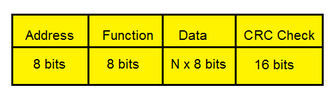
\includegraphics[width=.5\textwidth]{rtu_packet.png}
	\caption{Pacote da comunicação RTU}
	\label{fig:rtu_packet}
	%\source{Fornecido junto com os pontos}
\end{figure} 
\subsubsection{Modo de transmissão TCP}
O modo de transmissão TCP é uma aplicação do protocolo MODBUS baseado em TCP/IP, consequentemente utilizando a conexão ethernet. Para a pilha de comunicação, nesse protocolo é adicionado ao quadro um cabeçalho MBAP (MODBUS Application Protocol), deitando o modelo de mensagem como a figura \ref{fig:tcp_packet}:

\begin{figure}[h]
	\centering
	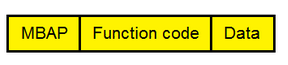
\includegraphics[width=.6\textwidth]{tcp_packet.png}
	\caption{Pacote da comunicação TCP}
	\label{fig:tcp_packet}
	%\source{Fornecido junto com os pontos}
\end{figure}
Esse novo cabeçalho tem 7 bytes de tamanho sendo composto por os seguintes elementos:
\begin{itemize}
	\item Transaction identifier: usado para identificação da resposta para a transação (2 bytes);
	\item Protocol identifier: 0 (zero) indica Modbus (2 bytes);
	\item Length: contagem de todos os próximos bytes (2 bytes);
	\item Unit identifier: utilizado para identificar o escravo remoto em uma rede Modbus RTU (1 byte).
	
\end{itemize}

O Modbus  TCP nao utiliza um byte de checkagem ao final da mensagem, pois o pŕoprio frame ethernet já apresenta uma checagem do tipo CRC-32. Na comunicação o cliente Modbus TCP inicia a conexão com o servidor para enviar as requisições, onde a porta padrão para a conexão com os servidores é a TCP 502.


\chapter{Medotologia}\label{cap:CnptDsng}

\section{Escolha da frequência}\label{sec:esc_freq}
A frequência foi escolhida com base no regulamento da Anatel. O mesmo estabelece que equipamentos de radiocomunicação com faixas restritas de: 902-907,5; 915-928; 2400-2483,5; 5725-5850 MHz, assim para os cálculos iniciais foi escolhida uma frequência de 920MHz.

\section{Estudo do Obstáculo}\label{sec:est_obs}
O primeiro passado adotado foi a análise dos pontos, verificando se entre os dois existia algum obstáculo. Essa informação pode ser extraída dos mapas que foram fornecidos em anexo, como mostra a figura \ref{fig:obs_cam}.
\begin{figure}[h]
	\centering
	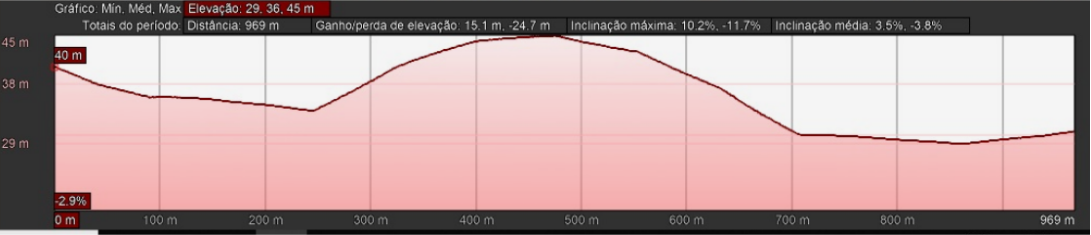
\includegraphics[width=1\textwidth]{obs_cam.png}
	\caption{Gráfico de obstáculo}
	\label{fig:obs_cam}
	%\source{Fornecido junto com os pontos}
\end{figure} 

Por meio da análise do gráfico, fica evidenciado que entre os dois pontos existe um grande obstáculo arredondado, assim sendo necessário calcular o seu raio de curvatura e a partir disso ver o quanto ele irá interferir na transmissão.
É feita uma aproximação do topo do obstáculo, utilizando uma curvatura parabólica como mostrado na figura 4 \ref{fig:obs_raio}.
\begin{figure}[h]
	\centering
	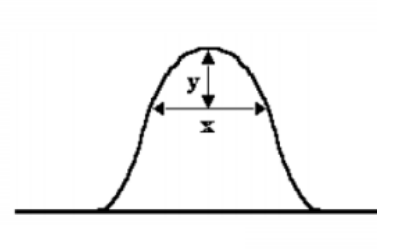
\includegraphics[width=.4\textwidth]{obs_raio.png}
	\label{fig:obs_raio}
	\caption{Curvatura parabólica utilizada para aproximação}
	%\source{Própria}
\end{figure} 

O raio $r$ da parábola será calculado o $\alpha$ que possibilita encontrar quantos decibéis de interferência o obstáculo irá causar. O cálculo do raio $r$ é feito utilizando a seguinte formula:
\begin{equation}
r = \dfrac{x^2}{8y}*10^{-3}
\end{equation}

Onde $x$ representa a distância em metros entre os dois pontos de igual nível, sendo um em cada lado do pico considerado e $y$ representa a diferença de cota entre o pico do obstáculo e a curva de nível considerada para  medida $x$.

\section{Atenuação do Obstáculo}
O cálculo do fator $\alpha$ relaciona a frequência $f$, o raio de curvatura da parábola $r$, a distância entre o vértice do obstáculo ao ponto de transmissão $d_1$ e a distância entre o vértice do obstáculo ao ponto de recepção $d_2$, ambas em \textit{Km}.
\begin{equation}
\alpha = 0,0818\dfrac{1}{\sqrt[6]{f}}\sqrt[3]{r}\sqrt{\dfrac{d_1+d_2}{d_1*d_2}}
\end{equation}

A atenuação é encontrada a partir de $\alpha$ e a relação entre os fatores  $H_c$ e $r_f$ por meio do gráfico 6. Onde $H_c$ representa a diferença entre ponto máximo do obstáculo e o nivelamento das antenas, enquanto $r_f$  é chamado de raio de \textit{fresnel}, sendo calculado com as mesmas distâncias $d_1$ e $d_2$. A relação é encontrada como mostrado na figura 6.

\begin{figure}[h]
	\centering
	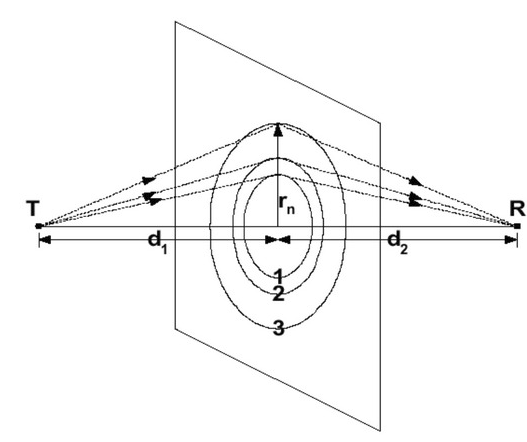
\includegraphics[width=.6\textwidth]{rf_img.png}
	\label{fig:rf_img}
	\caption{Modelo da zona de \textit{Fresnel}}
	%\source{Própria}
\end{figure}

O cálculo de $r_f$ se dá por:
\begin{equation}
r_f = \sqrt{\dfrac{n\lambda d_1 d_2}{d_1 + d_2}}
\end{equation}

\begin{figure}[h]
	\centering
	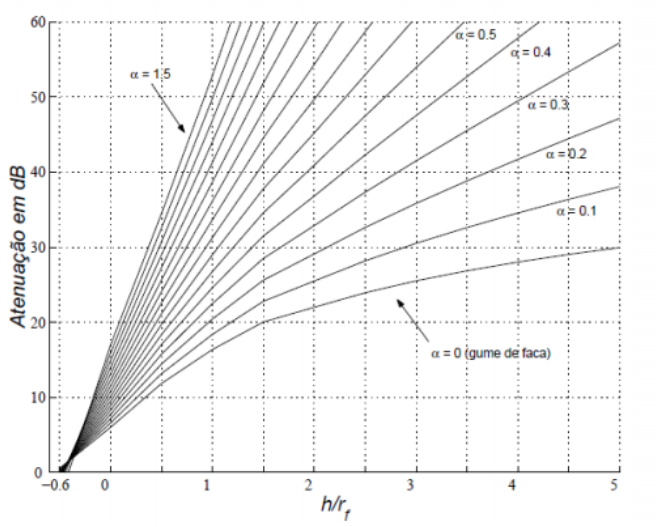
\includegraphics[width=.8\textwidth]{graf_ate.png}
	\label{fig:graf_ate}
	\caption{Gráfico de atenuação}
	%\source{Própria}
\end{figure} 


\begin{center}
	\begin{table}[]
		\begin{tabular}{|l|l|}
			\hline
			Rf    & 8,866 \\ \hline
			Hc    & 5     \\ \hline
			Hc/rf & 0,563 \\ \hline
		\end{tabular}
	\end{table}
\end{center}


\section{Atenuação no espaço livre}
O sinal também sofrerá atenuação ao ser transmitido no espaço livre, o cálculo da atenuação $L$ se dá por meio da fórmula de \textit{Fris}:
\begin{equation}
L = 32,45 +20(\log_{10}(d_1+d_2) + \log_{10}f)
\end{equation}



\section{Atenuação total}
A atenuação total é a soma da atenuação no espaço livre com a atenuação do obstáculo, assim :
\begin{equation}
L_{tot} = L + L_{obstaculo}
\end{equation}

\chapter{Resultados}
\section{Dados de entrada}
\subsection{Dados Gerais}
A altura escolhida para as torres foi de 0 e 9 para manter a linha de visada direta em paralelo com o chao e assim facilitando os cálculos e diminuindo os erros, os outros dados estão mostrados na tabela abaixo.
	\begin{table}[h]
		\centering
		\begin{tabular}{|
				>{\columncolor[HTML]{DAE8FC}}c |l|}
			\hline
			Distância Total (m) & 0,96713                  \\ \hline
			$\lambda$           & 0,001086957 x  $10^{-6}$ \\ \hline
			Altura das torres   & 0/9                      \\ \hline
		\end{tabular}
	\end{table}
\subsection{Dados dos Obstáculos}

\begin{table}[h]
	\centering
	\begin{tabular}{|
			>{\columncolor[HTML]{DAE8FC}}c |l|}
		\hline
		X                                                   & 325     \\ \hline
		Y                                                   & 7       \\ \hline
		$d_1$                                               & 0,475   \\ \hline
		\multicolumn{1}{|l|}{\cellcolor[HTML]{DAE8FC}$d_2$} & 0,49213 \\ \hline
	\end{tabular}
\end{table}
			
\section{Memorial de Cálculo}
\subsection{Frequência}
Não foi necessário calcular a frequência, o valor utilizado foi de 920MHz e sua escolha está justificada em \ref{sec:esc_freq}.

\subsection{Raio da Parábola}
Com os valores de $X$ e $Y$ do obstáculo o valor encontrado para o raio da parábola foi de:
\begin{equation}
	r_{parabola}= 1,886160714
\end{equation}

\subsection{Atenuação do obstáculo}
Com os valores de $d_1$ e $d_2$ o $\alpha$ encontrado teve valor de :
\begin{equation}
	\alpha = 0,6703932617
\end{equation}

O parâmetro $H_c$ foi encontrado por meio dos dados fornecidos, como mostrado na figura a seguir:
\begin{figure}[h]
	\centering
	\includegraphics[width=.8\textwidth]{hc.png}
	\label{fig:hc}
	\caption{Dados de $H_c$}
	%\source{Própria}
\end{figure} 

O parâmetro $r_f$ foi cálculado por meio da equação de $Fresnel$, com o valor dos parâmetros a seguir, foi encontrado no gráfico o valor da atenuação do obstáculo.

\begin{table}[h]
	\centering
	\begin{tabular}{|
			>{\columncolor[HTML]{DAE8FC}}c |l|}
		\hline
		$r_f$                                                         & 8,866    \\ \hline
		$H_c$                                                         & 5        \\ \hline
		$\dfrac{H_c}{r_f}$                                            & 0,563    \\ \hline
		\multicolumn{1}{|l|}{\cellcolor[HTML]{DAE8FC}$L_{obstaculo}$} & $22,5dB$ \\ \hline
	\end{tabular}
\end{table}

\subsection{Atenuação no Espaço livre}
Com os valores de $d_1$, $d_2$ e $f$ conhecidos o valor encontrado para $L$ foi:
\begin{equation}
L = 91,43dB
\end{equation}

\subsection{Atenuação total}
A atenuação total consiste nas soma das atenuação encontradas, logo:
\begin{equation}
L_{tot} = L + L_{obstaculo} = 91,43 + 22,5 = 113,9dB 
\end{equation} 

\section{Escolha do tranmissor e da antena}
 A escolha dos módulos e da antena se deu baseado na frequência escolhida para os cálculos e na versatilidade de cada dispositivo. 
 
 O modelo das antenas foi o \textit{Yagi(AirMax Antenna 900Mhz)},devido a sua faixa de trabalho e alta potência.
 
 O modelo do transmissor foi o \textit{Ubiquiti Networks(Rocket M9)} pot ser recomendado para trabalhar em conjunto com o modelo de antena \textit{Yagi}.
 \begin{figure}[h]
 	\centering
 	\includegraphics[width=.5\textwidth]{antena.jpeg}
 	\label{fig:antena}
 	\caption{Antena \textit{Yagi AirMax Antenna 900Mhz} }
 	\source{Ubiquiti Networks}
 \end{figure} 

\section{Receptor}
Escolha do receptor é encontrado à partir das potências das antenas, do módulo tranmissor e das perdas durante a transmissão. Sua potência foi calculada da seguinte forma:
\begin{equation}
	P_{receptor} = P_{antena_tx} + P_{antena_rx} + P_{transmissor} - L_{tot}
\end{equation}

A mesma antena utilizada para transmissão é utilizada para recepção, os dados da sua potência estão disponíveis nos seu \textit{datasheet} onde $P_{antena_{tx}} = P_{antena_{rx}} = 19dBi$. A potência do transmissõr também está disponível no datasheet, onde $P_{transmissor} = 28dBm$. O valor encontrado para potência do receptor foi de $	P_{receptor} = -47.9dBi$

Com o valor de $-47.9dBi$, o módulo \textit{Ubiquiti Networks(Rocket M9)} também poderá ser utilizado para recepção, tornando o sistema mais simplificado já que ambos receptores e transmissores estarão utilizando antenas recomendadas no datasheet.

\newpage
\begin{center}
	\Large \textbf{Variáveis do projeto}
\end{center}
Todos os valores utilizados e calculados estão registrados na figura a seguir:
\begin{figure}[h]
	\centering
	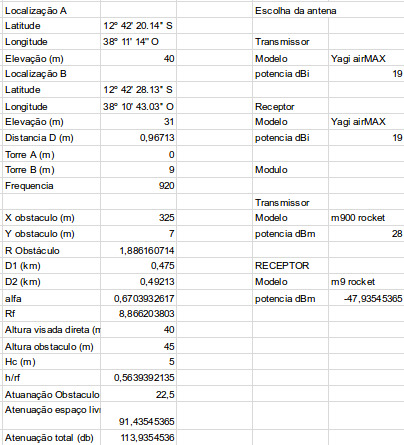
\includegraphics[width=1\textwidth]{resultados.jpeg}
	\label{fig:result}
	\caption{Variáveis do projeto}
	%\source{Própria}
\end{figure} 




%\chapter{Conclusão e Trabalhos Futuros}\label{cap:conclusao}

\lipsum[82-84]

\section{Trabalhos Futuros}

\lipsum[85] 

% ----------------------------------------------------------
% ELEMENTOS PÓS-TEXTUAIS (Referências, Glossário, Apêndices)
% ----------------------------------------------------------
\postextual

\begin{center}
	\Large \textbf{Referências}
\end{center}
	
	[1] TUDE, Eduardo. Enlace rádio digital ponto a ponto. 2004.

% Referências bibliográficas
%\bibliography{bibliografia}

%\printglossaries




% Índice remissivo (Consultar manual)
%\phantompart
%\printindex



\end{document}
